\capitulo{5}{Aspectos relevantes del desarrollo del proyecto}

En este apartado, se van a detallar los aspectos más interesantes del desarrollo del proyecto y los desafíos a los que me he tenido que enfrentar a lo largo del mismo. 

Además, es importante detallar las decisiones que se tomaron en esos momentos de dificultad e indicar de qué manera se solventaron los problemas.

Por otro lado, también voy a indicar en este apartado cual es la arquitectura general del sistema diseñado dado que me parece que es un aspecto interesante dentro del proyecto.

\section{Análisis de las webs de extracción de datos}
En las primeras fases del proyecto, se realizó un análisis de las webs de las Universidades públicas de Castilla y León para estudiar cuales podrían ser los atributos de interés para mostrar en la web del proyecto. Durante este proceso, surgieron varios problemas para la obtención de información. Esto se debió a que cada universidad subía las convocatorias a su web con un formato particular y con unos datos e informaciones particulares. Esto es un problema a la hora de querer montar una web de convocatorias centralizada dado que uno de los aspectos más importantes de una web es la uniformidad de la misma. A continuación, se van a comentar algunos de los desafíos que fueron encontrados durante esta fase.

\subsection{Universidad de Salamanca}
Debido a mi poco conocimiento en cuanto a las convocatorias PDI y PAS, en primer lugar se realizó \textit{web scraping} de un portal de la USAL en el que se publicaban todas las convocatorias pero en el que no se tenía conocimiento si una convocatoria estaba en plazo o no. Esto se debe a que las fechas que comprendían el plazo no estaban publicadas en páginas web sino en documentos PDF. 

Se planteó la posibilidad de realizar PDF scraping de las convocatorias de esta universidad pero tras tiempo de investigación, se descubrió que estos ficheros no seguían un formato unificado.  Finalmente, debido a la imposibilidad de recopilación de datos de la web de la USAL ~\cite{usal:latex} debido a la falta de datos necesarios para la web a desarrollar, se decidió excluir esta universidad del proyecto.

\subsection{Universidad de León}
El realizar el raspado de datos de esta universidad, también fue un reto en el proyecto. Esta universidad mostraba algunas convocatorias en plazo mientras que en verdad ya no estaban abiertas a candidatos (Por ejemplo, ya se habían publicado los listados de admitidos) ~\cite{ule:latex}. Para determinar si una oferta estaba en plazo o no, la única manera era mediante la examinación de los títulos de los PDF adjuntos a una determinada convocatoria. Para ello, se realizó una estructura de datos con las palabras no deseadas con aquellas palabras que, en el caso de localizar alguna en un título ya sabíamos que esa convocatoria no estaba en plazo. 

Esto llevo largos tiempos de análisis para finalmente tan solo acabar detectando las convocatorias que estaban en plazo verdaderamente. Es posible, que en casos futuros, vuelvan a surgir convocatorias fuera de plazo que están detectadas como que si lo son. Para ello, es necesario que si se continúa con el desarrollo de la aplicación, se tenga muy en cuenta este aspecto.

A continuación se va a mostrar un ejemplo en el que se da este caso. En la siguiente imagen, se va a exponer una convocatoria que actualmente está en plazo:

\begin{figure}[H]
    \centering
    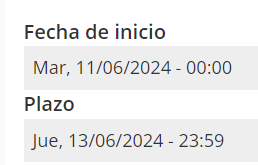
\includegraphics[width=0.4\linewidth]{DocumentacionTFG//img/ConvocatoriaEnPlazoULE.PNG}
    \caption{Convocatoria en plazo ULE}
    \label{fig:enter-label}
\end{figure}

Sin embargo, si nos fijamos en el archivo adjunto a esa convocatoria, aparecerá una resolución de aprobados, lo cual quiere decir que la convocatoria no está en plazo.

\begin{figure}[H]
    \centering
    
\includegraphics[width=0.75\linewidth]{DocumentacionTFG//img/FicheroAdjuntoULE.PNG}
    \caption{Fichero Adjunto a Convocatoria}
    \label{fig:enter-label}
\end{figure}

Con la implementación de la estructura de datos de las palabras no deseadas, esta convocatoria no sería elegida.

\subsection{Universidad de Valladolid}
Al realizar \textit{web scraping} de las páginas web en las que se muestran las convocatorias PDI Y PAS de la Universidad de Valladolid ~\cite{uva:latex}, también surgieron una serie de imprevistos. Esto se debe a que había convocatorias que aparecen en esta web cuyo estado indicaba que estaba 'EN PLAZO' pero si nos fijamos en las fechas de las mismas en verdad no lo están.

\begin{figure}[H]
    \centering
    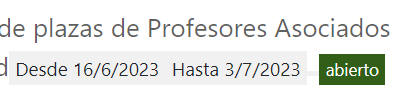
\includegraphics[width=0.75\linewidth]{DocumentacionTFG//img/EjemploConvocatoriaIncorrectaUVA.PNG}
    \caption{Estado Convocatoria Incorrecto}
\end{figure}

Esto fue algo que no percibí en la primera etapa del proyecto, posteriormente, decidí arreglarlo para que las ofertas se mostrasen en plazo con exactitud mediante la comparación de las fechas del plazo con la fecha actual.

Otro de los problemas, fue que, en numerosas convocatorias de la Universidad de Valladolid, había campos vacíos, esto hizo que en algunas convocatorias que por ejemplo no indicaban cuales eran su fecha de inicio de plazo y su fecha de fin, se tuviesen que determinar por cerradas.

\begin{figure}[H]
    \centering
    
\includegraphics[width=0.75\linewidth]{DocumentacionTFG//img/CamposVaciosUVA.PNG}
    \caption{Convocatorias con campos vacíos}
\end{figure}

Estos han sido algunos inconvenientes a la hora de recopilar los datos de las distintas universidades. Todos ellos se han tratado de solventar de la manera más lógica posible intentando que afecten de la manera más mínima a la idea de aplicación que se tenía en el inicio.

\section{Integración con Calendario Personal}

Para añadir funcionalidad extra a la aplicación, se decidió realizar una integración con Google Calendar, para ello, en primer lugar, se tenía que dar la posibilidad a los usuarios de iniciar sesión con Google. Esto se implementó mediante la autenticación basada en OAuth 2.0 lo cual permitía a los usuarios de mi aplicación web iniciar sesión mediante la utilización de las cuentas de Google ~\cite{oauth2:latex}. 

Posteriormente, cuando el proceso de autenticación estaba completado, se realizó un desarrollo para que los usuarios pudiesen añadir como evento, las fechas de fin de las convocatorias a Google Calendar desde la aplicación y de esta manera disponer de un recordatorio previo antes de que las convocatorias expirasen. Esta integración se intentó realizar mediante Google Cloud Console que permitía a los desarrolladores gestionar sus servicios en Google Cloud.

Esta integración con Google y Google Calendar, se acabó llevando a cabo y era funcional para usuarios de test, sin embargo, si se quería publicar la aplicación y que la integración fuese funcional para cualquier usuario, Google requería lo siguiente para completar el proceso de verificación:

\begin{itemize}
    \item Un enlace oficial a la Política de Privacidad de la aplicación
    \item Un vídeo de YouTube que muestra cómo 
 se planea utilizar los datos de usuario de Google que obtiene de los ámbitos.
    \item Una explicación escrita que le indique a Google por qué necesita acceso a datos de usuario confidenciales y/o restringidos.
    \item Todos tus dominios verificados en Google Search Console
\end{itemize}

Estas restricciones, fueron consideradas demasiado duras como para un proyecto de este calibre. Además, quizás esta integración limitaba el disfrute de la funcionalidad de la aplicación para aquellos usuarios que no dispusiesen de cuenta de Google, por lo tanto se decidió cambiar esta funcionalidad y se implementó un nuevo sistema de avisos por correo.

\textbf{Nuevo Sistema de Avisos por Correo}

Para este sistema de avisos implementado, los usuarios no tenían necesariamente que iniciar sesión con su cuenta de correo electrónico de manera inicial como anteriormente. 

Para la utilización de esta funcionalidad, bastará con que el usuario se suscriba al sistema de avisos de la convocatoria que el desee mediante un formulario en el que debe introducir su correo electrónico. 

Una vez que se suscribe, le llegará al usuario un correo con información de la convocatoria solicitada y un archivo ICalendar definido por la aplicación. Estos archivos permiten añadir como evento a su calendario personal la fecha de fin de una convocatoria para que el usuario se acuerde del fin de plazo de la misma. Además, en este caso dará igual cual sea el servicio de correo electrónico utilizado (Google, Outlook...) lo cual mejora enormemente la implementación anterior.

\section{Despliegue de la aplicación}

La idea inicial para realizar el despliegue de la aplicación, era Docker ~\cite{docker:latex}. Esta es una herramienta que permite a los desarrolladores a crear, compartir, ejecutar y verificar aplicaciones en cualquier lugar sin complejas configuraciones del entorno. 

Sin embargo, cuando se utiliza Docker en Windows, es necesario tener habilitada alguna tecnología de virtualización, normalmente el Subsistema de Windows para Linux. Para ello, se necesita habilitar la característica WSL en mi ordenador lo cual era una operación que no acababa de completarse debido a errores en el camino. 

Tras varias pruebas, cambios en archivos de configuración, etc. Se decidió investigar otras herramientas para el despliegue. Esta decisión tomada, es algo que ha dado un salto de calidad al proyecto debido a que actualmente la aplicación está desplegada de una manera muy profesional y novedosa.

Los componentes fundamentales para el despliegue final de la aplicación han sido los siguientes:
\begin{itemize}
    \item \textbf{Servidor de Azure Database para MySQL: ~\cite{azuremysql:latex}} En este servidor en la nube, se ha desplegado la base de datos MySQL. Esta decisión se ha tomado de esta manera debido a la facilidad que nos proporciona Azure para realizar despliegues sin realizar tareas de infraesctructura.
    \item \textbf{GitHub Action:~\cite{githubactions:latex}} Esta herramienta es utilizada para la automatización de flujos de trabajo. En el sistema, se ha utilizado esta herramienta para crear una tarea programada que ejecutará el proyecto en Python y por lo tanto hará que la base de datos se actualice de manera periódica.
    \item \textbf{Azure App Services: ~\cite{azureappservices:latex}} Este es un servicio basado en HTTP que permite hospedar aplicaciones web en la nube. En nuestro sistema, es el encargado de lanzar y alojar la aplicación desarrollada en .NET en la nube. Esto fue sencillo debido a que tanto Azure como .NET son propias de Microsoft por lo tanto el despliegue se pudo realizar con facilidad. Para que la información de la base de datos se mostrase correctamente en la web desplegada, se tuvieron que configurar las variables de entorno de este App Service e introducir la cadena de conexión de la base de datos desplegada en el servidor Azure Database. Este fue el último paso del montaje de la arquitectura del sistema y por lo tanto ya estaba la aplicación funcional disponible para utilizarse. 
\end{itemize}

\newpage
\begin{landscape}
\subsubsection{Diagrama de arquitectura general del sistema desplegado}
\vspace{2cm}
\imagenapaisada{DiagramaGeneralArquitectura}{Diagrama arquitectura general del sistema.}\label{img-diagrama-general}   
\end{landscape}
\newpage








